\chapter{Colouring}
\label{ch:colouring}
\index{graph colouring|textbf}

This chapter and the next complete Part~III's third family. Chapter~\ref{ch:hittingset}
minimised a set subject to a covering constraint; Chapter~\ref{ch:cover}
tightened the constraint and found the algorithm that solves it. Colouring
keeps the hard constraint and drops the minimisation: there is nothing to
optimise, only a question of whether a configuration exists at all.

It is also the place where a promise made in Chapter~\ref{ch:potts} comes due.
Proper colouring is the antiferromagnetic $q$-state Potts model at zero
temperature --- this book's own model at the opposite sign --- so if the
machinery is what it has been claimed to be, the colouring calculation should be
a substitution and not a new theory. It is, and the substitution produces two
closed forms.

One is a surprise. For proper colouring, the transmission of a complex does not
depend on its cardinality at all: a clique of nine members transmits exactly what
a single edge does. The other is the opposite: for the weaker hypergraph
constraint the transmission collapses like $q^{-c}$, and by cardinality four a
complex has almost stopped constraining anything. Identical at cardinality two,
these two problems diverge violently above it, and
Sec.~\ref{sec:twoconstraints-col} is why.

\section{Colouring as a hard-core problem}
\label{sec:colouringdef}

Give every node one of $q$ colours and forbid an edge whose endpoints agree.
There is no chemical potential and no ground-state energy to minimise: a
colouring either exists or it does not, and the question is at what density of
constraints it stops existing.

In the language of Chapter~\ref{ch:statmech} this is
Eq.~\eqref{eq:emitted} with an interior that assigns weight zero to forbidden
configurations and weight one to the rest. Nothing else changes. What does
change, before any algebra, is the \emph{message}. Up to now a message has been one number --- a probability, a field, an integer, or
at worst three states. Here it is a distribution over $q$ colours,
$\eta_{i\to a}(\sigma)$, and there is no ferromagnetic direction to project it
onto. That is the sense in which colouring is heavier than anything before it,
and Sec.~\ref{sec:colouring-scalar} is the observation that rescues it.

\paragraph{Two constraints, not one.} On a graph there is only one way to
forbid, but on a chygraph a complex of $c$ members admits two natural rules and
they are not the same.

\emph{Proper colouring} of the induced graph: every pair inside a complex is an
edge, so all $c$ members must take \emph{distinct} colours. This needs $q\ge c$
and is what one means by colouring a clustered graph whose motifs have been
promoted to complexes.

\emph{Hypergraph colouring}: only a \emph{monochromatic} complex is forbidden.
Two members may agree as long as not all of them do. This is the standard
higher-order generalisation, and it is strictly weaker.

At $c=2$ the two coincide, which is exactly why the distinction has no
counterpart on a graph. Above it they are different problems, and
Chapter~\ref{ch:cover}'s pairing of hitting set with vertex cover was the same
distinction one family earlier: how much of a complex may be left alone.

\section{What a complex transmits}
\label{sec:colouring-scalar}
\index{transmission factor}

The uniform assignment $\eta\equiv1/q$ is always a fixed point --- every colour
equally likely everywhere, which is the replica-symmetric solution. Linearise
about it and one number governs the result.

\begin{calculation}{one number, because the colours are interchangeable}
Write $\eta_{j}=1/q+w_{j}$ with $\sum_{\sigma}w_{j}(\sigma)=0$, which is forced
because both $\eta$ and $1/q$ are normalised. The perturbations therefore live
in the $(q-1)$-dimensional traceless subspace, and permuting the colours is a
symmetry of the whole problem. By Schur's lemma the linearised map acts on that
subspace as a \emph{scalar}. So although the message carries $q-1$ numbers, its
linearisation carries one, and Chapter~\ref{ch:statmech}'s branching matrix
applies unchanged with that scalar in place of $u'$. This is checked directly:
three different traceless directions return one number.

\emph{Proper colouring.} The emitted quantity is
\[
  Z(\sigma_{0})=\!\!\sum_{\substack{\sigma_{1}\dots\sigma_{c-1}\ \text{distinct}\\
    \text{and all}\ \ne\sigma_{0}}}\ \prod_{j}\eta_{j}(\sigma_{j}).
\]
Differentiate with respect to $\eta_{1}(s)$. The result is zero unless
$s\ne\sigma_{0}$, and when $s\ne\sigma_{0}$ it is the same quantity $A$ for
every such $s$, because the remaining sum depends only on how many colours have
been excluded and not on which. So the linear response is
\[
  \sum_{s}w_{1}(s)\,A\,\mathbf{1}[s\ne\sigma_{0}]
  =A\Bigl(\sum_{s}w_{1}(s)-w_{1}(\sigma_{0})\Bigr)=-A\,w_{1}(\sigma_{0}),
\]
the first sum vanishing by tracelessness. With
$A=q^{2-c}(q-2)!/(q-c)!$ and $Z_{0}=q^{1-c}(q-1)!/(q-c)!$ at the uniform point,
the ratio $A/Z_{0}=q/(q-1)$, and after normalising,
\begin{equation}
  \tau_{c}(q)=-\frac{1}{q-1}.
  \label{eq:taucol}
\end{equation}
Every combinatorial factor cancels. The cardinality has gone.

\emph{Hypergraph colouring.} Here the constraint removes a single configuration,
so
\[
  Z(\sigma_{0})=1-\prod_{j}\eta_{j}(\sigma_{0}),
\]
and expanding the product to first order gives, after the same normalisation,
\begin{equation}
  \tau^{\mathrm{hyp}}_{c}(q)=-\frac{1}{q^{\,c-1}-1}.
  \label{eq:tauhyp}
\end{equation}
At $c=2$ this is Eq.~\eqref{eq:taucol}, as it must be.
\end{calculation}

Both forms are confirmed by enumerating the interior exactly, in rational
arithmetic, so the agreement is an identity rather than a numerical
coincidence.

Figure~\ref{fig:colouring} draws both, and the contrast is the chapter in one
picture: three cardinalities lying exactly on top of one another for the proper
rule, and fanning out over three decades for the hypergraph one.

\paragraph{Why the cardinality cancels, in words.} What one member
of a clique learns from another is a single fact: \emph{not that colour}. It
learns the same fact from every other member. Because the perturbation is
traceless --- the colours have to keep summing to one --- excluding one colour
is the whole of the information, and excluding it again from a second member
adds nothing to the linear response. A clique of nine transmits what an edge
transmits.

The negative sign is not decoration either. Colouring is an
\emph{antiferromagnet}: raising the probability of a colour at one node lowers
it at the next. Chapter~\ref{ch:statmech} warned that the sign of the entries,
not of the leading eigenvalue, is what classifies a map, and this is the third
map in the book whose entries are negative --- after the hard-field maps of
Chapters~\ref{ch:hittingset} and~\ref{ch:cover}.

\begin{figure}[t]
\centering
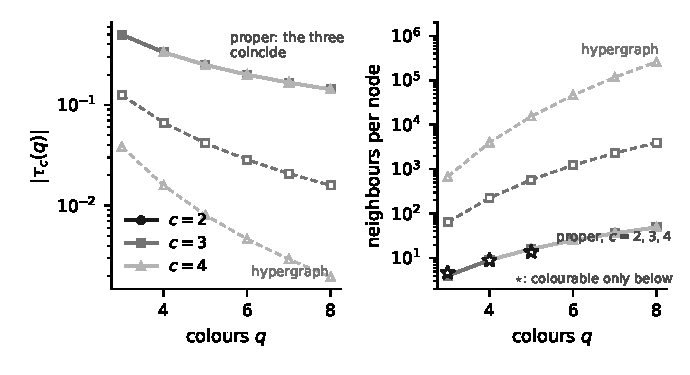
\includegraphics[width=\linewidth]{figs/fig-colouring.pdf}
\caption{\textbf{Two constraints, identical at cardinality two.} Left: the
transmission of a complex, Eqs.~\eqref{eq:taucol} and~\eqref{eq:tauhyp}. For
proper colouring (solid) the three cardinalities fall exactly on top of one
another, each curve starting at $q=c$ since a smaller palette admits no proper
colouring at all; for hypergraph colouring (dashed) the transmission collapses
like $q^{-c}$. Right: the resulting local-stability threshold in neighbours per
node. Proper colouring sits at $(q-1)^{2}$ whatever the cardinality --- the
graph value; hypergraph colouring runs away as $(q^{c-1}-1)^{2}$. Stars are the
published colourability thresholds for Erd\H{o}s--R\'enyi graphs
\citep{mulet2002}, which lie \emph{below} the stability line for $q\ge4$: see
Sec.~\ref{sec:colouring-rsb}. Generated by \code{figs/colouring.py}.}
\label{fig:colouring}
\end{figure}

\section{The threshold, and what it is}
\label{sec:colouringthreshold}
\index{de Almeida--Thouless line}

Substituting into Eq.~\eqref{eq:branch} needs one decision, and it is the
decision Chapter~\ref{ch:ising} already made in Sec.~\ref{sec:atline}.

There is no ordered phase to look for here: the uniform solution \emph{is} the
replica-symmetric solution, and what one asks is whether a perturbation of
\emph{random sign} grows. That perturbation is transmitted with $\tau$ and its
effect measured by squaring, so the operative condition is the de
Almeida--Thouless form --- $\ave{u'}$ replaced by $\ave{u'^{2}}$ everywhere,
which by Eq.~\eqref{eq:reweight} is an elementwise reweighting and nothing more.
For a single layer,
\begin{equation}
  \ave{\kbar}\,(c-1)\,\tau_{c}^{2}=1.
  \label{eq:colthresh}
\end{equation}

\paragraph{The graph case, against the literature.} Put $c=2$, where a complex
is an edge and the chy-degree is the ordinary degree. What is left to choose is
the degree distribution. For a \emph{Poisson} one, $\ave{\kbar}=\ave{k}$ ---
a Poisson distribution being its own excess --- and Eq.~\eqref{eq:colthresh}
gives $\ave{k}=(q-1)^{2}$. For a \emph{regular} one, a node of degree $k$ has
$k-1$ other edges, so $\ave{\kbar}=\ave{k}-1$ and it gives
$\ave{k}=(q-1)^{2}+1$. Both are
Ref.~\citep{zdeborova2007}'s Eq.~(18), which reads
$c_{\mathrm{RS}}^{\mathrm{ER}}=q^{2}-2q+1$ and
$c_{\mathrm{RS}}^{\mathrm{reg}}=q^{2}-2q+2$; the stability analysis and its
large-$q$ asymptotics are worked out in Ref.~\citep{krzakala2004}, and the
replica treatment of the same ensemble in Ref.~\citep{vanmourik2002}.

Two published expressions from one $\tau$, and the difference between them is
exactly the excess-degree convention this book has been carrying since
Sec.~\ref{sec:map}. That is the check the chapter needed, and it is a stronger
one than a single number would have been, because a formalism that had the
excess bookkeeping wrong would reproduce at most one of the two lines.

\paragraph{Cardinality, and the two constraints.} Now raise it. Counting in
\emph{neighbours} per node --- a complex of cardinality $c$ supplies $c-1$ of
them --- Eq.~\eqref{eq:colthresh} gives
\begin{equation}
  \text{proper: } (q-1)^{2},
  \qquad
  \text{hypergraph: } \bigl(q^{\,c-1}-1\bigr)^{2}.
  \label{eq:coltwo}
\end{equation}
The first does not move. A network of $c$-cliques loses stability at exactly the
same number of neighbours per node as a graph does, for every cardinality and
every $q$: promoting motifs to complexes changes nothing at all here. The second
runs away --- at $q=4$ it is $9$, $225$, $3969$ for $c=2,3,4$.

The second is not new, and the agreement is a check rather than a result.
Reference~\citep{gabrie2017} solves $q$-colouring of $K$-uniform random
hypergraphs and its Eq.~(43) gives the same linear-stability bound,
$\ell^{\mathrm{RS}}_{\mathrm{stab}}=(q^{K-1}-1)^{2}/(K-1)$ for a Poisson degree
of mean $\ell$ --- which is $(q^{c-1}-1)^{2}$ neighbours per node, this
chapter's Eq.~\eqref{eq:coltwo}. Its Appendix~B derives the transmission at
finite temperature and Eq.~\eqref{eq:tauhyp} is that expression at
$\beta\to\infty$. What is left to this chapter is the first line and the
contrast: that the same substitution gives both rules, and that they part
company only above cardinality two.

The first of these is the same phenomenon as Eq.~\eqref{eq:kc}, which found
$\ave{k}(c-1)=e$ for hitting set: counted in neighbours, hyperedge size does not
move the point. Two hard-core problems, two different constants, one structure.
The reason is the same both times --- what a complex transmits and how many
neighbours it supplies move in exactly compensating ways. This is the
\emph{opposite} of the Ising model, where Sec.~\ref{sec:clustering} found the two effects failing to compensate and
the multiplicity winning.

\section{The two constraints diverge above cardinality two}
\label{sec:twoconstraints-col}

Equation~\eqref{eq:coltwo} says the following.

Proper colouring of a clique network is, at this level of description,
indistinguishable from colouring a graph with the same number of neighbours.
Hypergraph colouring of the same object is not remotely the same problem: a
cardinality-four complex over four colours tolerates $3969$ neighbours per node
where the proper constraint tolerates $9$.

The gap is entirely a matter of how much a complex forbids. A clique of four
rules out all but $q(q-1)(q-2)(q-3)$ of $q^{4}$ assignments; the monochromatic
rule leaves all but $q$ of them. At $c=2$ those are the same statement and the
distinction is invisible --- which is why it has no name in the graph
literature, and why it needed a formalism with cardinality in it to become
visible.

This is the third time Part~III has found a distinction that exists only above
cardinality two. Section~\ref{sec:hardfail} found the hard-field limit exact at
$c=2$ and wrong above it; Sec.~\ref{sec:corefree} found the core-free branch
present at $c=2$ and absent above it; and here two constraints coincide at $c=2$
and separate by three orders of magnitude above it. The pattern is not a
coincidence. Cardinality two is degenerate in a specific way --- a complex with
two members has no room for a partial violation --- and a great deal of what
looks like general theory is an artefact of working there.

\section{A graph with triangles}
\label{sec:colouring-triangles}

Cardinality independence has a consequence the previous section did not draw,
and it is the one case where the chapter's constraint and the book's running
comparison meet.

For \emph{proper} colouring a triangle-clustered graph is not a new object at
all. A triangle forbids its three members from agreeing pairwise, which is what
its three edges already say, so the problem is ordinary $q$-colouring of an
ordinary graph and the graph calculation applies to it. Put a regular network in
which every vertex sits in $\kappa$ triangles, so that its degree is $n=2\kappa$
and the triangles meet only at vertices. Then Eq.~\eqref{eq:colthresh} on the
chygraph of triangles gives $\ave{\kbar}(c-1)=2(\kappa-1)=n-2$, while the same
network read as a graph of degree $n$ gives $\ave{\bar k}=n-1$. The two answers
are
\begin{equation}
  \text{chygraph: } n=(q-1)^{2}+2,
  \qquad
  \text{graph: } n=(q-1)^{2}+1,
  \label{eq:tridisagree}
\end{equation}
and they disagree by one in degree at every $q$.

The chygraph is the right one, for the reason the book has been giving since
Sec.~\ref{sec:treelike}. The graph calculation adds the messages arriving at a
vertex as though its neighbours were independent; inside a triangle two
neighbours are adjacent, and the three edges close a loop. Promoting the
triangle to a complex puts that loop inside Eq.~\eqref{eq:emitted}, where it is
summed exactly, and leaves a structure over triangles that really is treelike.
The graph answer is not an approximation that happens to be close --- it is off
by exactly the one branch the loop costs.

\paragraph{Both ends of one formula.} Nothing above required dropping a layer.
Take links and triangles together at fixed degree, with $a$ the link chy-degree,
$b$ the triangle chy-degree, $n=a+2b$, and $f=2b/n$ the fraction of degree
carried by triangles. Because $\tau$ does not depend on cardinality, both layers
carry the same $s=\tau^{2}=(q-1)^{-2}$, and the two-layer determinant of
Eq.~\eqref{eq:LT} reads
\begin{equation}
  s\,(n-3)+2s^{2}\bigl[n(1-f/2)-1\bigr]=1 .
  \label{eq:trifamily}
\end{equation}
At $f=0$ this returns $(q-1)^{2}+1$ and at $f=1$ it returns $(q-1)^{2}+2$,
exactly and in rational arithmetic, with the cross term doing all of the
interpolating. The two lines of Eq.~\eqref{eq:tridisagree} are one formula at
its two ends.

\paragraph{How big is it, honestly.} One in degree, and only for regular
ensembles. For Poisson layers $\ave{\kbar}=\ave{\kappa}$, the cross term
$\ave{\kappa}_{|}\ave{\kappa}_{\triangle}-\ave{\kbar}_{|}\ave{\kbar}_{\triangle}$
vanishes identically, and Eq.~\eqref{eq:trifamily} returns $(q-1)^{2}$ at every
$f$: there is no difference at all. So this is not a statement that clustering
moves the colouring threshold. It is the regular ensemble's lost branch, the
same one that separates $(q-1)^{2}$ from $(q-1)^{2}+1$ in
Sec.~\ref{sec:colouringthreshold}, arriving where it can be mistaken for
physics. Chapter~\ref{ch:ising} found clustering worth $13.9$ per cent in
$T_{c}$ and Sec.~\ref{sec:helporhurt} found it worth a fifth of $q_{c}$; here it
is worth one in degree, and for half the ensembles nothing.

That is the third sign the book has taken on this comparison, and the least
dramatic of them. It is included because the cheap conclusion --- that a
formalism built for higher-order structure must find higher-order structure
mattering --- is wrong, and the arithmetic that shows it is wrong is three
lines.

\section{Where replica symmetry goes}
\label{sec:colouring-rsb}
\index{replica symmetry breaking}

Now the qualification, and it is a large one. Colouring is the classic
one-step replica-symmetry-breaking problem, and Eq.~\eqref{eq:colthresh} is not
a one-step answer. So it is important to say precisely what it is and, more
importantly, what it is not; Sec.~\ref{sec:colouring-sp} then does the
calculation it is not.

It is the point where the replica-symmetric solution loses \emph{local}
stability --- where the spin-glass susceptibility diverges. It is not the
colourability threshold. Comparing with the published Erd\H{o}s--R\'enyi values
\citep{mulet2002} gives Table~\ref{tab:colpublished}.
\begin{table}[t]
\centering\small
\begin{tabular}{rrrr}
\hline\hline
$q$ & $(q-1)^{2}$ & clustering $c_{d}$ & colourable to $c_{q}$\\
\hline
$3$ & $4$ & $4.42$ & $4.69$\\
$4$ & $9$ & $8.27$ & $8.90$\\
$5$ & $16$ & $12.67$ & $13.69$\\
\hline\hline
\end{tabular}
\caption{\textbf{A local stability line is not a colourability line.} Eq.~\eqref{eq:colthresh} at cardinality two against the published Erd\H{o}s--R\'enyi clustering and colourability thresholds \citep{mulet2002}. At $q=3$ the instability sits inside the colourable phase; from $q=4$ upward it sits above the colourability threshold, so it is on the wrong side rather than merely loose.}
\label{tab:colpublished}
\end{table}

At $q=3$ the local instability sits inside the colourable phase, below both the clustering
transition and the colourability threshold. At $q=4$ and above it sits
\emph{above} the colourability threshold --- the graph has long since stopped
being colourable by the time the replica-symmetric solution notices anything is
wrong. The criterion is not merely loose there; it is on the wrong side.

That is not a defect of the chygraph construction. It is the known behaviour of
replica-symmetric colouring, and Ref.~\citep{zdeborova2007} records it in the
same words: the instability threshold lies in the colourable phase only for
$q=3$. What this chapter contributes is that the same statement, with the same
constants, comes out of the general branching matrix; and that it extends to
complexes, where Eq.~\eqref{eq:coltwo} says a clique network behaves exactly like
a graph and a hypergraph does not.

\paragraph{What is needed instead.} The colourability threshold requires the
one-step calculation --- survey propagation and the iterative algorithms built
on it \citep{braunstein2003,mulet2002}, and a complexity function. The next
section does that much. What it does not do is the condensation and rigidity
transitions Ref.~\citep{zdeborova2007} maps out, or the rigorous side of the
same question \citep{cojaoghlan2016}.

Whatever it returns, Eq.~\eqref{eq:coltwo} remains a statement about the
stability of a particular solution and not about when colourings run out --- and
the interesting part of it, that cardinality drops out of the proper constraint
and dominates the hypergraph one, is a statement about the interior sum that a
one-step treatment inherits unchanged, because Eqs.~\eqref{eq:taucol}
and~\eqref{eq:tauhyp} are properties of a complex and not of an ansatz.

\section{Surveys, and colourability}
\label{sec:colouring-sp}
\index{survey propagation|textbf}
\index{replica symmetry breaking}

Table~\ref{tab:colpublished} has three columns and the chapter has so far
produced one of them. This section produces the other two, and it produces them
by redoing a published calculation rather than by extending one. Survey
propagation for colouring is Refs.~\citep{braunstein2003,mulet2002}', the
thresholds it returns are theirs, and nothing below is a new result. It is here
because a book that spends a chapter saying its own threshold is the wrong line
should be able to compute the right one, and because the machinery is then in
place for cardinalities above two, where Sec.~\ref{sec:colouring-sp-chy} takes
it.

The object one level up is a survey: a distribution, over the clusters of
colourings, of the colour a node is forced to. Colour symmetry does most of the
work of carrying it. A survey is uniform over colours, so one scalar per
inclusion suffices --- $e$, the probability that a node is forced at all, with
each colour taking $e/q$ of it.

What symmetry does \emph{not} do is decouple the colours, and this is the whole
of the calculation. A forced neighbour forbids exactly one colour, so ``every
colour but one is forbidden'' is a question about whether $q-1$ colours are
\emph{covered} by the forced neighbours, not a product of $q-1$ independent
events. Inclusion--exclusion over which colours are missed gives
\begin{equation}
  \begin{split}
    P(\text{only }c\text{ free})&=\sum_{j=0}^{q-1}(-1)^{j}\binom{q-1}{j}
      \prod_{k}\Bigl(1-\frac{e_{k}(1+j)}{q}\Bigr),\\
    P(\text{none free})&=\sum_{j=0}^{q}(-1)^{j}\binom{q}{j}
      \prod_{k}\Bigl(1-\frac{e_{k}j}{q}\Bigr),
  \end{split}
  \label{eq:colsp}
\end{equation}
the product running over the other neighbours, and the survey update being the
first divided by one minus the second --- the contradictory state discarded, as
in Sec.~\ref{sec:sat-sp}. Treating the colours as independent instead is the
obvious shortcut and it is wrong; it is caught by asking for three thresholds
rather than one.

The complexity is Eq.~\eqref{eq:sigma} with one term fewer, a graph having no
complexes above cardinality two to sum over:
\begin{equation}
  \Sigma=\bigl\langle\ln\bigl(1-P(\text{none free})\bigr)\bigr\rangle
        -\frac{\ave{k}}{2}\Bigl\langle\ln\Bigl(1-\frac{e_{i}e_{j}}{q}\Bigr)
        \Bigr\rangle,
  \label{eq:colsigma}
\end{equation}
the edge term being the weight of two ends not forced to the same colour.

\begin{table}[t]
\centering\small
\begin{tabular}{rccr}
\hline\hline
$q$ & $\Sigma=0$ at & $c_{q}$ published & error\\
\hline
$3$ & $4.683\,(0.012)$ & $4.69$ & $-0.1\%$\\
$4$ & $8.901\,(0.012)$ & $8.90$ & $+0.0\%$\\
$5$ & $13.660\,(0.008)$ & $13.69$ & $-0.2\%$\\
\hline\hline
\end{tabular}
\caption{\textbf{The colourability threshold, computed.} Where the complexity of
Eq.~\eqref{eq:colsigma} vanishes, against Mulet's $c_{q}$
\citep{mulet2002}. Bracketed figures are the spread over three seeds. Compare
the $(q-1)^{2}$ column of Table~\ref{tab:colpublished}: $4$, $9$ and $16$ against
these. Generated by \code{figs/colouring.py}.}
\label{tab:colsp}
\end{table}

Table~\ref{tab:colsp} is the result. Set beside Table~\ref{tab:colpublished} it
says what Sec.~\ref{sec:colouringthreshold} could not: at $q=4$ the stability
line sits at $9$ and the colourings run out at $8.90$, so the replica-symmetric
solution is still locally stable after the problem has become unsolvable, and
the size of that error is now a number rather than a direction.

The clustering threshold arrives without further work, though less sharply. The
density at which the surveys stop being trivial --- below which no cluster
forces anything and $e$ collapses to zero --- is $c_{d}$, and it comes out of
the same population that gives $\Sigma$: $4.46$ against a published $4.42$ at
$q=3$, and $8.49$ against $8.27$ at $q=4$. That is a per cent and then three,
against a tenth of a per cent for $c_{q}$, and the asymmetry is the expected
one. A vanishing complexity is a crossing and can be bisected; a branch
appearing is a fold, and a population of twenty thousand locates it less well.
Both remaining columns of Table~\ref{tab:colpublished} nonetheless come from one
calculation, with neither used in getting there.

\paragraph{The same three qualifications.} They are
Sec.~\ref{sec:sat-sp}'s and they apply here unchanged: this is $m=0$, so the
condensation and rigidity transitions are outside it; the treelike condition of
Eq.~\eqref{eq:up} is untouched; and reproducing published constants is a check
on the implementation, not a result. To say it once more, since a section that
computes five-figure agreement can be mistaken for one that discovers
something: every number in Table~\ref{tab:colsp} was already known. What the
chygraph adds is that Eqs.~\eqref{eq:colsp} and~\eqref{eq:colsigma} are written
for an arbitrary chy-degree distribution and an arbitrary interior, which is
what makes the next section a substitution rather than a second derivation.

\section{Above cardinality two, and what the rule costs}
\label{sec:colouring-sp-chy}
\index{survey propagation}

The previous section stayed at $c=2$, where the chygraph is a graph and the
answer was already known. This section raises the cardinality, and the interest
is not in the numbers --- those are known too --- but in which of the two rules
survives the step and which does not.

\paragraph{What a complex has to tell a member.} In the hard-field limit the
message from a complex is the set of colours it forbids the member it is
speaking to. Everything about how that message combines with the others at a
node turns on one question: \emph{how many colours can a single complex forbid
at once?}

For the hypergraph rule the answer is \textbf{at most one}. A complex is
violated only when all of its members share a colour, so it can forbid $\gamma$
to member $0$ only when every one of the other $c-1$ members is already forced
to $\gamma$ --- and they cannot all be forced to two different colours at the
same time. The message is therefore the same \emph{kind} of object as at
cardinality two, a single forbidden colour or none, and Eq.~\eqref{eq:colsp}
carries over with one substitution: the weight $e/q$ that a neighbour forbids a
given colour becomes $h/q$, where
\begin{equation}
  h=q\prod_{j=1}^{c-1}\frac{e_{j}}{q}
  \label{eq:hypsp}
\end{equation}
is the weight that the complex forbids anything at all. Nothing else in the
node update changes, and the inclusion--exclusion of
Sec.~\ref{sec:colouring-sp} is reused unaltered.

For the proper rule the answer is \textbf{up to $c-1$}. Every member forced to a
different colour removes a different colour from member $0$, so a complex of
cardinality five can arrive carrying four prohibitions at once. The message is
no longer a colour but a \emph{set} of them, the events ``$\gamma$ is
forbidden'' and ``$\gamma'$ is forbidden'' are correlated within a single
complex as well as across complexes, and the node update needs the joint
distribution of the forbidden set rather than a scalar. Equation~\eqref{eq:colsp}
does not carry over, and no substitution repairs it.

That asymmetry is Sec.~\ref{sec:twoconstraints-col} again, one level up. There
the two rules were found to coincide at cardinality two and to separate above
it, in what they transmit. Here they coincide at cardinality two and separate
above it in something harder: whether the one-step machinery can be reused at
all. A complex with two members has no room for a partial violation, and it also
has no room to forbid two things at once; both statements are the same
degeneracy, and it is the second that decides how much work the next calculation
is.

\paragraph{Carrying it out.} Put Eq.~\eqref{eq:hypsp} into
Eq.~\eqref{eq:colsp}. The complexity of Eq.~\eqref{eq:colsigma} gains the one
term a graph does not have: a complex is violated when all $c$ of its members
agree, so it contributes
$\ln\bigl[1-q\prod_{j\le c}(e_{j}/q)\bigr]$, and there are
$\ave{k}/c$ complexes per node.

\begin{table}[t]
\centering\small
\begin{tabular}{ccccr}
\hline\hline
$q$ & $c$ & $\Sigma=0$ at & published & error\\
\hline
$3$ & $3$ & $26.900\,(0.000)$ & $26.92$ & $-0.07\%$\\
$4$ & $3$ & $63.276\,(0.024)$ & $63.30$ & $-0.04\%$\\
$2$ & $5$ & $52.283\,(0.043)$ & $52.32$ & $-0.07\%$\\
\hline\hline
\end{tabular}
\caption{\textbf{Hypergraph colouring above cardinality two.} Mean chy-degree at
which the complexity vanishes, against the colourability thresholds of
Ref.~\citep{gabrie2017}, Table~1. Bracketed figures are the spread over three
seeds. The three errors agree in sign and size, which is a converged bias of the
finite population rather than scatter. Generated by \code{figs/colouring.py}.}
\label{tab:hypsp}
\end{table}

Table~\ref{tab:hypsp} is the result.

The three rows are Ref.~\citep{gabrie2017}'s colourability thresholds, and the
agreement is a check on the substitution and not a new result: that paper solves
this problem, and Sec.~\ref{sec:colouringthreshold}'s hypergraph threshold is
its Eq.~(43). What the check establishes is that Eq.~\eqref{eq:hypsp} is the
whole of the difference --- that once a complex can forbid at most one colour,
cardinality enters the one-step calculation through a single scalar and through
nothing else.

\paragraph{Two exclusions, both real.} At $q=2$ with $c=3$ and $c=4$
Ref.~\citep{gabrie2017} marks its colourability threshold as invalid, the $m=0$
solution being unstable to noise propagation there. The calculation above will
return a number for those cases and it would mean nothing; they are omitted from
the table for that reason and not because they disagree. And the proper rule is
absent from the table because of the paragraph above, not because it was tried
and failed: a set-valued survey is a different calculation, and this book does
not do it.

\section{Checks}
\label{sec:colouring-checks}

\emph{Against enumeration, exactly.} Equations~\eqref{eq:taucol}
and~\eqref{eq:tauhyp} are checked against a direct enumeration of the interior
of a complex, in rational arithmetic so that the agreement is exact rather than
numerical: proper colouring for $q=3,\dots,7$ at every cardinality from $2$ to
$\min(q,5)$, and hypergraph colouring for $q=3,4,5$ at cardinalities $2$, $3$
and $4$.

\emph{That one number suffices.} The claim that the linearised map acts as a
scalar on the traceless subspace is checked by perturbing along three different
traceless directions and requiring the same answer, for both rules.

\emph{Against the literature.} Equation~\eqref{eq:colthresh} at $c=2$ returns
$(q-1)^{2}$ for a Poisson degree distribution and $(q-1)^{2}+1$ for a regular
one, which are the two lines of Ref.~\citep{zdeborova2007}'s Eq.~(18). The published thresholds of
Ref.~\citep{mulet2002} are quoted alongside, and the chapter states that they
lie below the stability line for $q\ge4$ rather than leaving that to be
discovered.

\emph{What is not checked, because it is not claimed.} Nothing here is a
colourability threshold. This chapter computes where a replica-symmetric
solution stops being locally stable, and Sec.~\ref{sec:colouring-rsb} is the
account of the difference.
